\section{Introduction}
\label{sec:introduction}
\IEEEPARstart{T}{iniTapeout}
TinyTapeout~\cite{tinytapeout} is an educational project that makes it easier and cheaper than ever to get ASIC designs manufactured.
The digital design flow consists of templating a GitHub~\cite{github} repository, adding a design, waiting for the tests and binary layout files (GDS~\cite{gds}) generation to complete, then submitting to a quarterly shuttle.

Up to 500 designs are multiplexed to 24 general purpose input/output (GPIO) pins, and after manufacture the chips are mounted to a demonstration board for easy testing.
Each design can be activated and tested in turn.
Documentation submitted with each project forms a printable datasheet~\cite{datasheet} as well as an online index at TinyTapeout.com/runs/~\cite{tinytapeoutruns}

Design entry is done mostly with Verilog or Wokwi~\cite{wokwi}.
Wokwi is a web based schematic based editor that is an easy way to get started for people with no prior hardware description language (HDL) experience.
The TinyTapeout website includes a basic getting started guide for drawing circuits with Wokwi available in English and Spanish.

The first~\cite{firstshuttle} free and experimental shuttle with 152 designs was submitted to the seventh Google sponsored~\cite{googlesponsored} lottery multi project wafer (MPW) shuttle in September 2022.
The next 4 shuttles combined 582 designs and were sponsored by and manufactured with the Efabless~\cite{efabless} chipIgnite MPW service.

\begin{table*}[htbp]
\centering
\caption{Table shows the stats for each of the TinyTapeout shuttle runs.}
\label{tab:tinytapeout}
\begin{tabularx}{\textwidth}{@{}l *{6}{X}@{}}
\toprule
\textbf{Run} & \textbf{Launched} & \textbf{Closed} & \textbf{Shuttle} & \textbf{Designs} & \textbf{Chips Expected} & \textbf{Estimated delivery date} \\
\midrule
TT01 & 2022-08-17 & 2022-09-01 & MPW7  & 152 & 2024-01-30 & Not expecting to ship this test \\
TT02 & 2022-11-09 & 2022-12-02 & 2211Q & 165 & 2023-10-17 & 2024-01-30 \\
TT03 & 2023-03-01 & 2023-04-23 & 2304C & 249* & 2024-01-15 & 2024-02-28 \\
TT04 & 2023-07-01 & 2023-09-08 & 2309  & 143 & 2024-02-28 & 2024-04-15 \\
TT05 & 2023-09-11 & 2023-11-04 & 2311  & 174 & 2024-04-12 & 2024-05-12 \\
TT06 & 2024-02-01 & 2024-04-19 & 2404  & TBD & TBD        & TBD \\
\bottomrule
\end{tabularx}
\end{table*}

Each tile is approximately $100\times 160 um$, enough for around 1000 logic gates and is priced at \$50.
The physical chip and demo board are optional and cost an additional \$250.
Individuals pay a reduced \$100 for their first chip and board thanks to sponsorship by Efabless\cite{efabless}.

By separating the cost of area and the cost of the chip, a group of 10 could submit 10 designs and share 1 board for \$600.

The GitHub templates\cite{verilogtemplate} make use of GitHub Actions\cite{githubactions} - an automatic continuous integration system that is triggered every time the repository is updated.
There are 4 main jobs:

\begin{enumerate}
	\item GDS - installs OpenLane and the Sky130 process design kit (PDK), then builds the GDS, and generates a summary of the design that includes utilization, standard cells used, and a 2D and 3D model of the GDS.
This job can optionally also run a gate-level verification.
	\item Verification - installs the YosysHQ open source CAD suite which includes many common electronic design automation (EDA) tools.
Then iVerilog and cocotb are used to run any testbenches included.
	\item Documentation - generates a preview of the documentation.
	\item Precheck - a number of tests are run to make sure that the design doesn’t cause design rule check (DRC) errors after integration into the chip.
\end{enumerate}

Successful GDS, Documentation, and Precheck jobs are required to submit to a shuttle.
Verification is optional but highly encouraged. Wokwi designs can make use of an integrated truth table testing system\cite{automatedtesting}.

While the process can be done entirely in the browser, it’s also possible to install a local copy of the tools, which can help to reduce iteration time, especially for tests and verification.

\begin{figure}[htp]
\centering
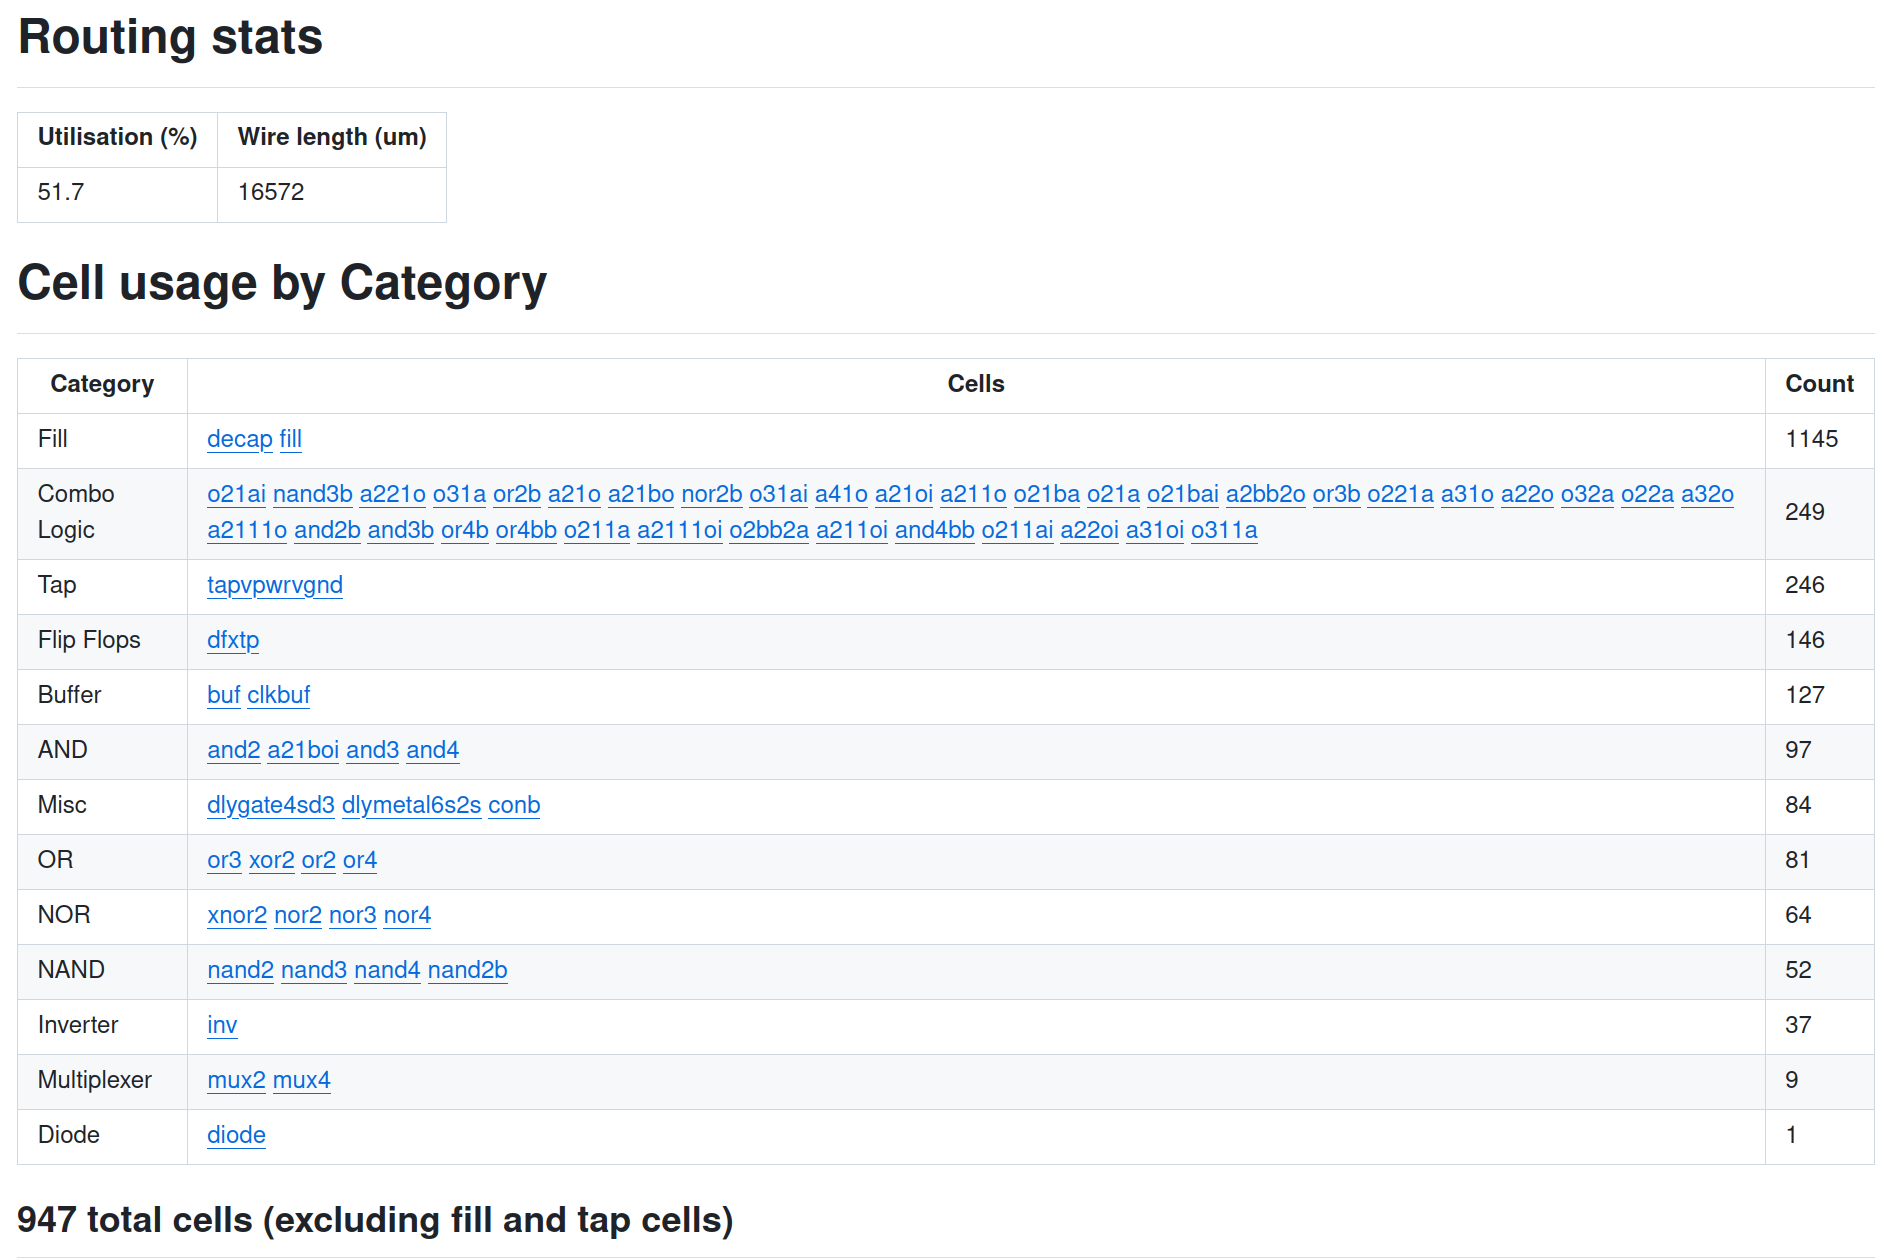
\includegraphics[width=\columnwidth]{./Figs/gh action cell stats.png}
\caption{The summary table of the GDS job.}
\label{fig:summary_table_GDS_job}
\end{figure}

\begin{figure}[htp]
\centering
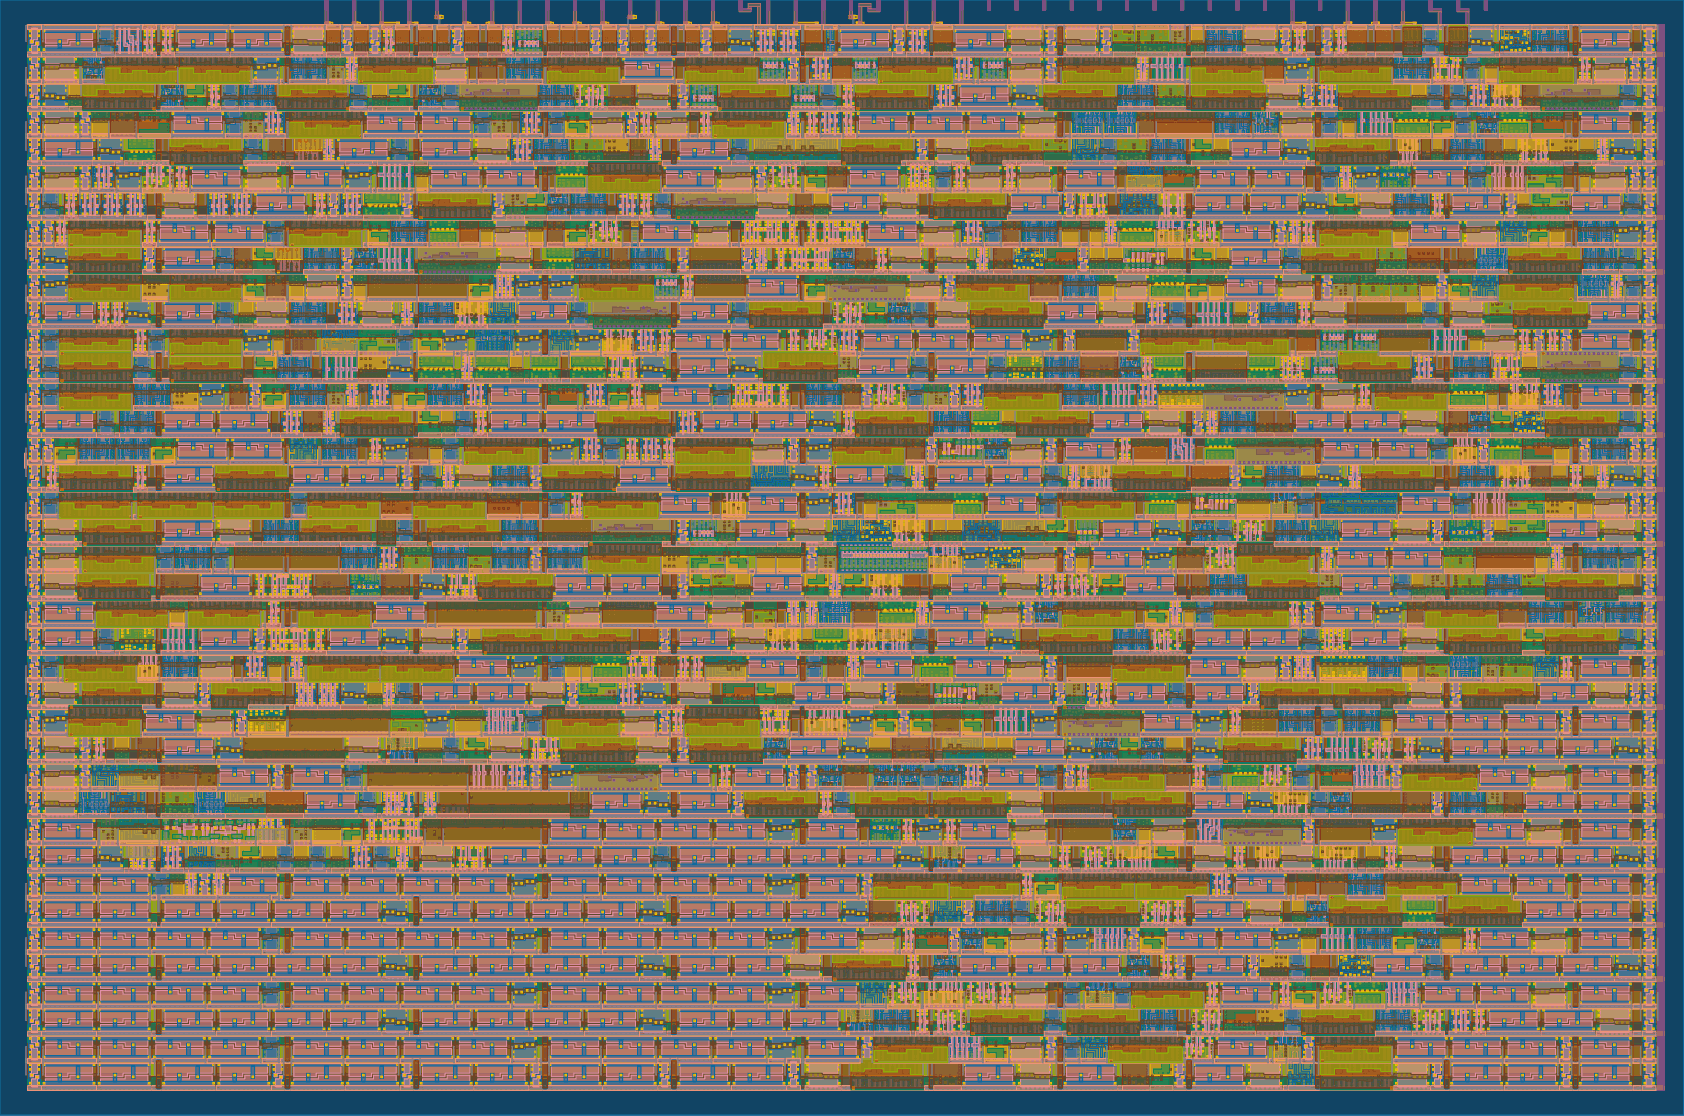
\includegraphics[width=\columnwidth]{./Figs/gh action gds layout.png}
\caption{The 2D render of the cells in use, with empty areas visible in the lower left corner.}
\label{fig:render_cells_in_use}
\end{figure}

\begin{figure}[htp]
\centering
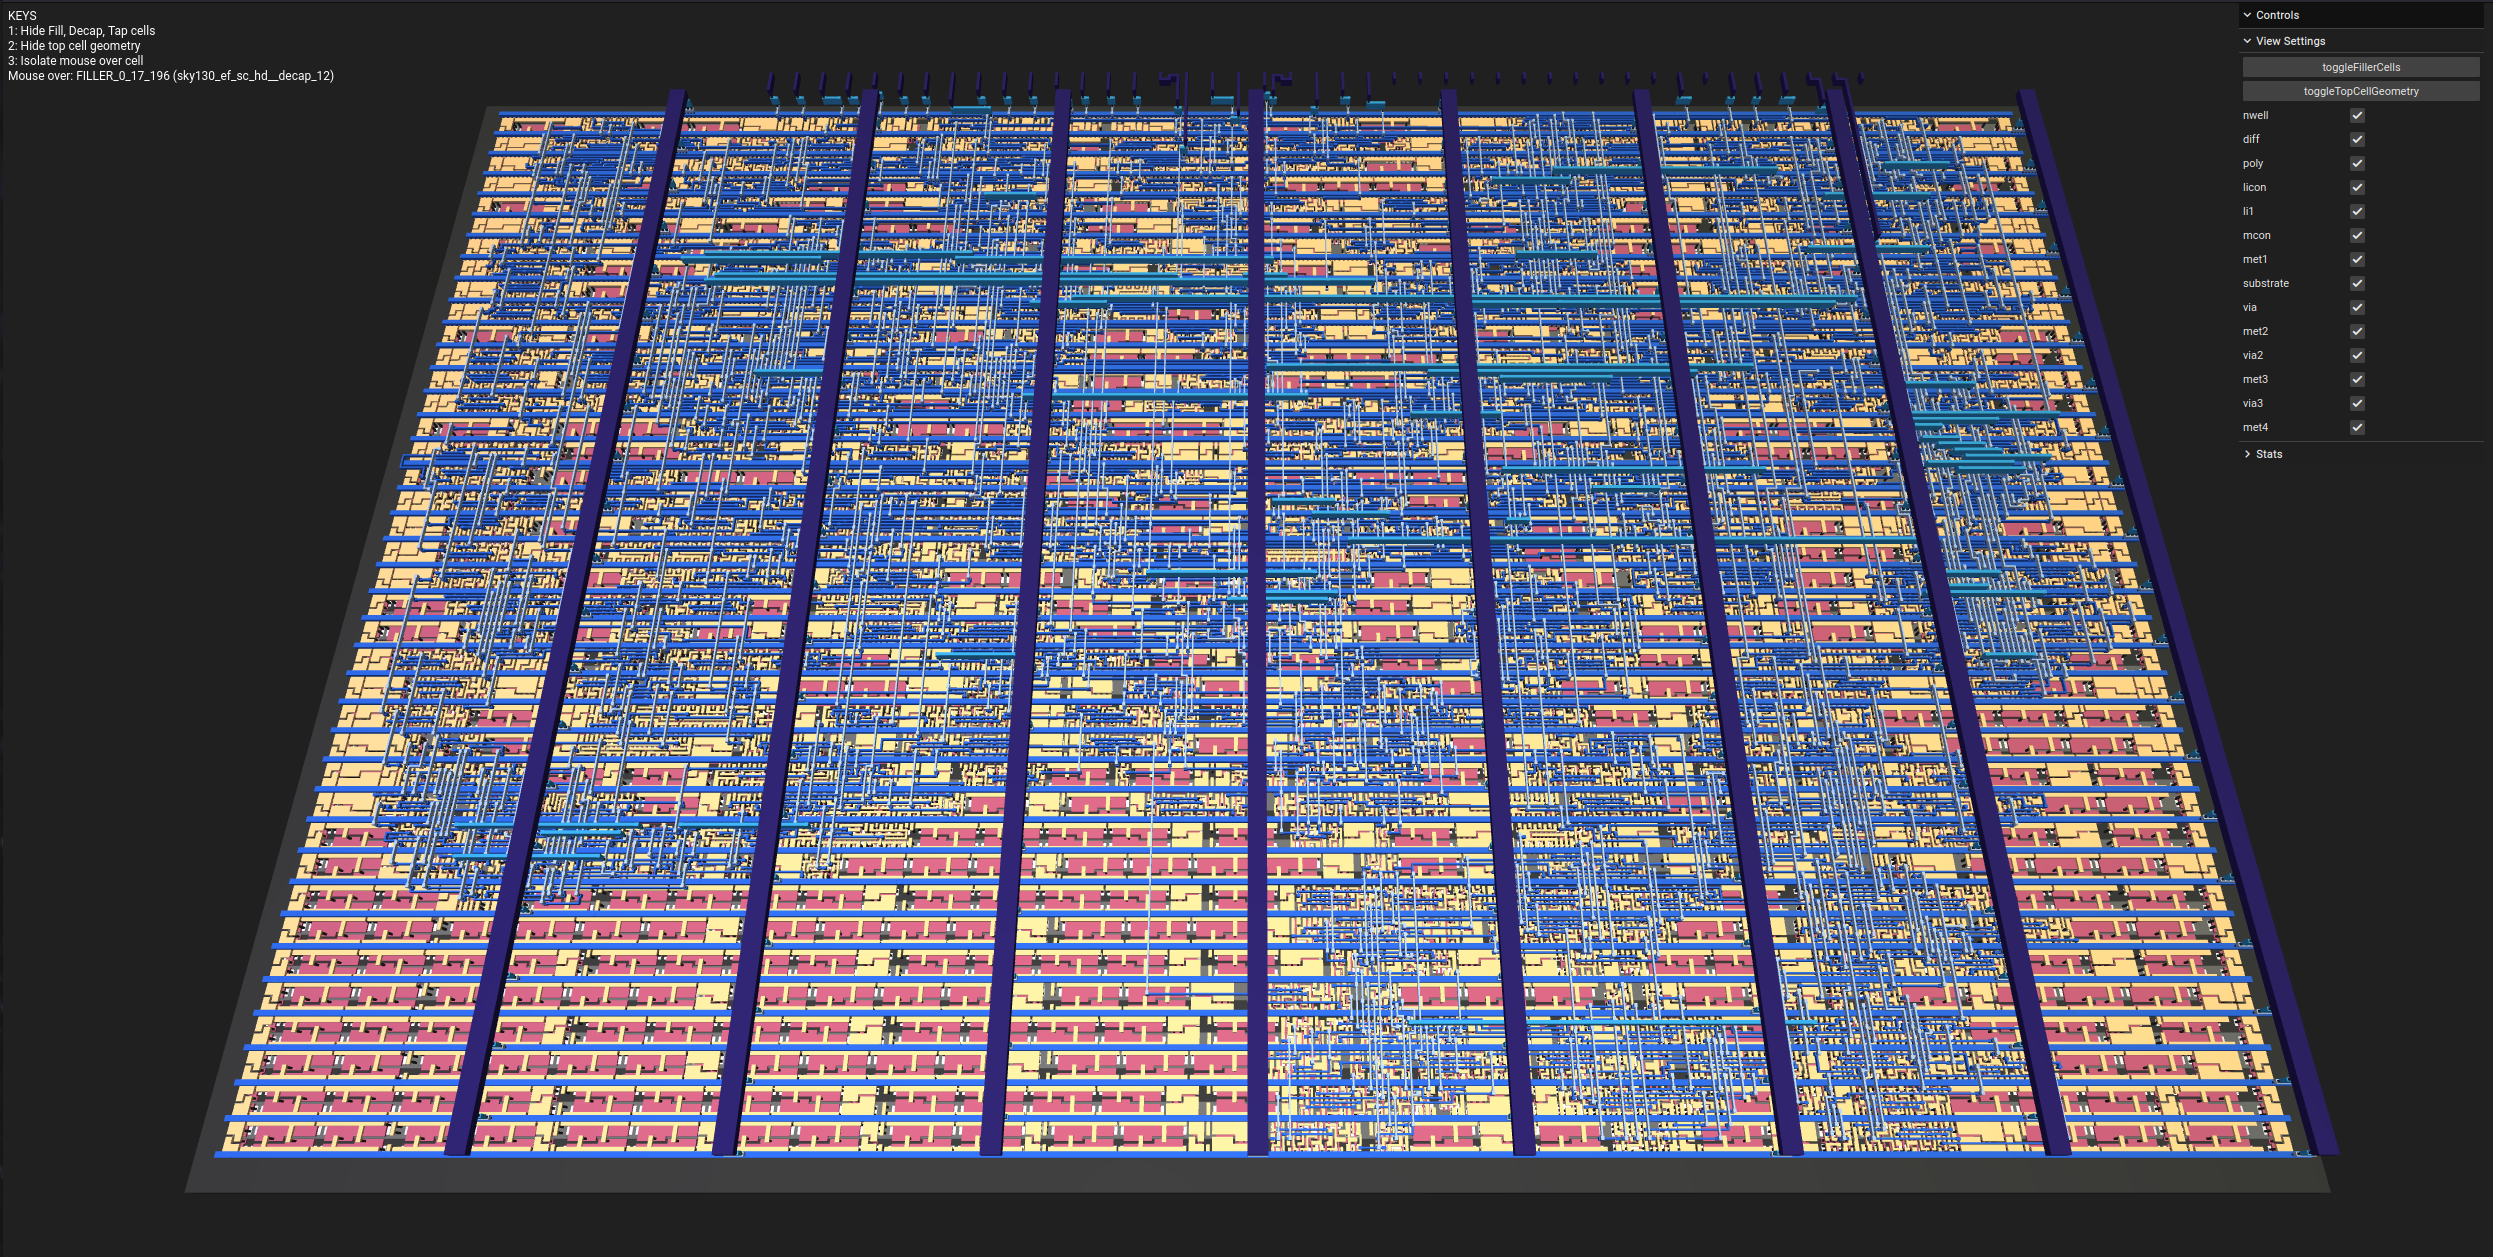
\includegraphics[width=\columnwidth]{./Figs/gh action gds 3d view.png}
\caption{The interactive 3D viewer.}
\label{fig:interactive_3D_viewer}
\end{figure}

\begin{figure}[htp]
\centering
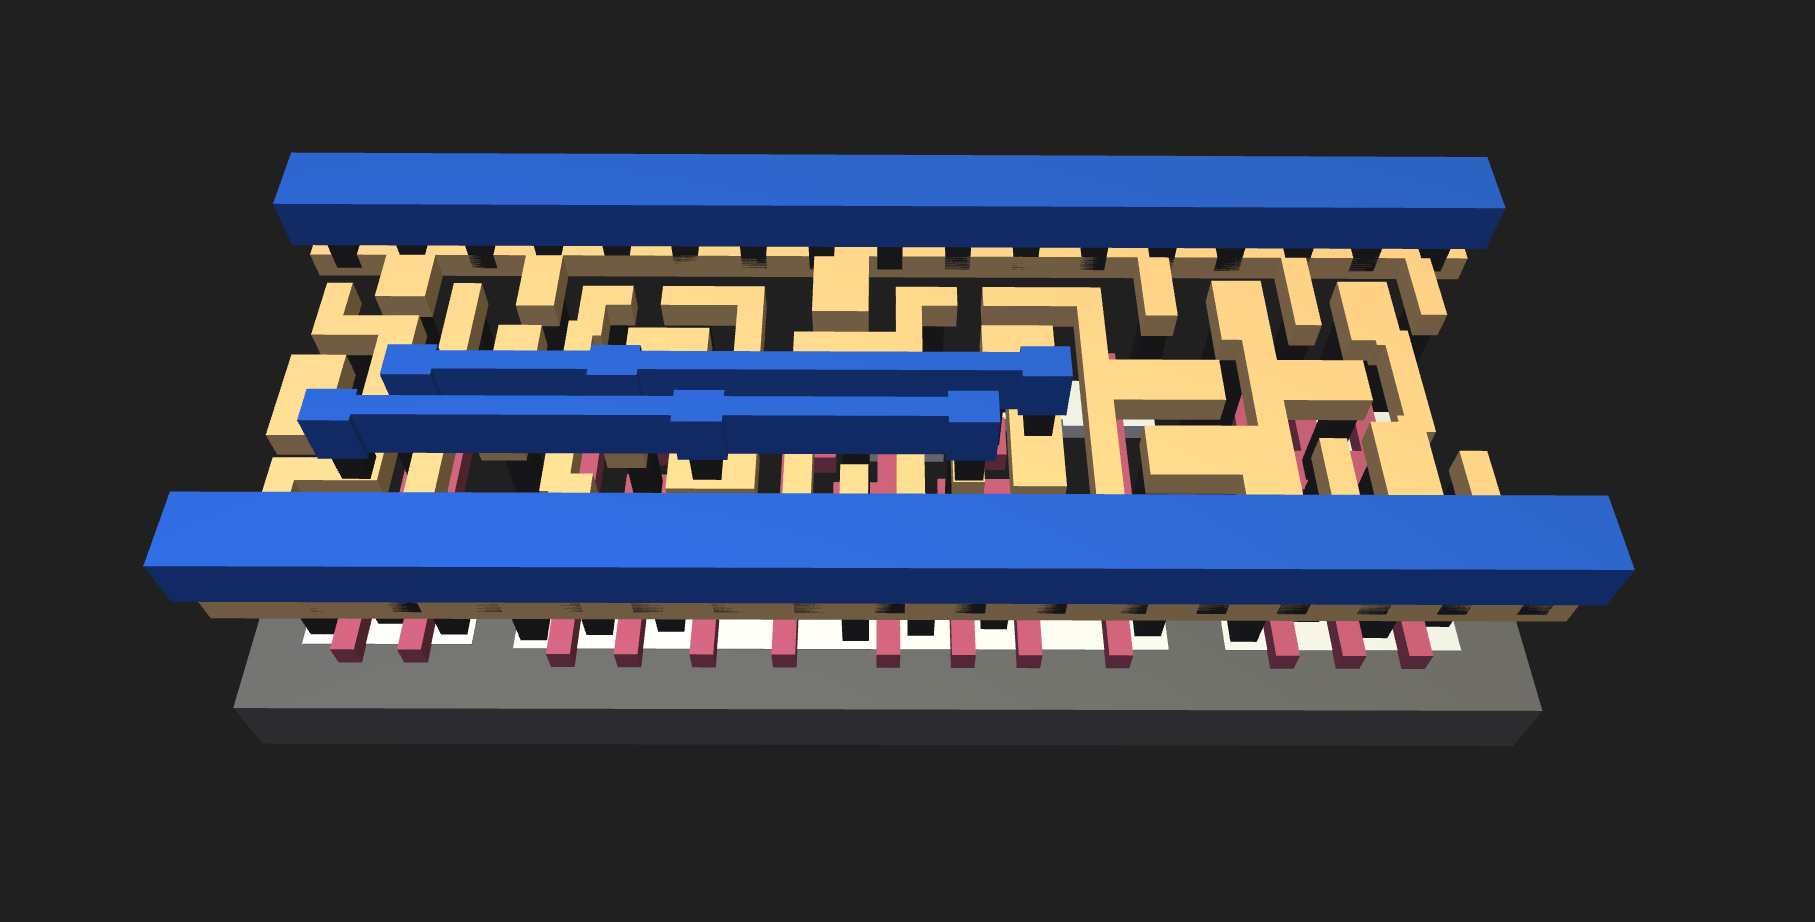
\includegraphics[width=\columnwidth]{./Figs/gh action d type flop 3d closeup.png}
\caption{A deep zoom to a D-type flip-flop, isolated from the rest of the design.}
\label{fig:zoom_d_flip_flop}
\end{figure}

Community engagement has been strong with 756 designs submitted over the 5 shuttles.
The Discord community has 1000 members with 1600 subscribed to the mailing list.

\begin{figure}[htp]
\centering
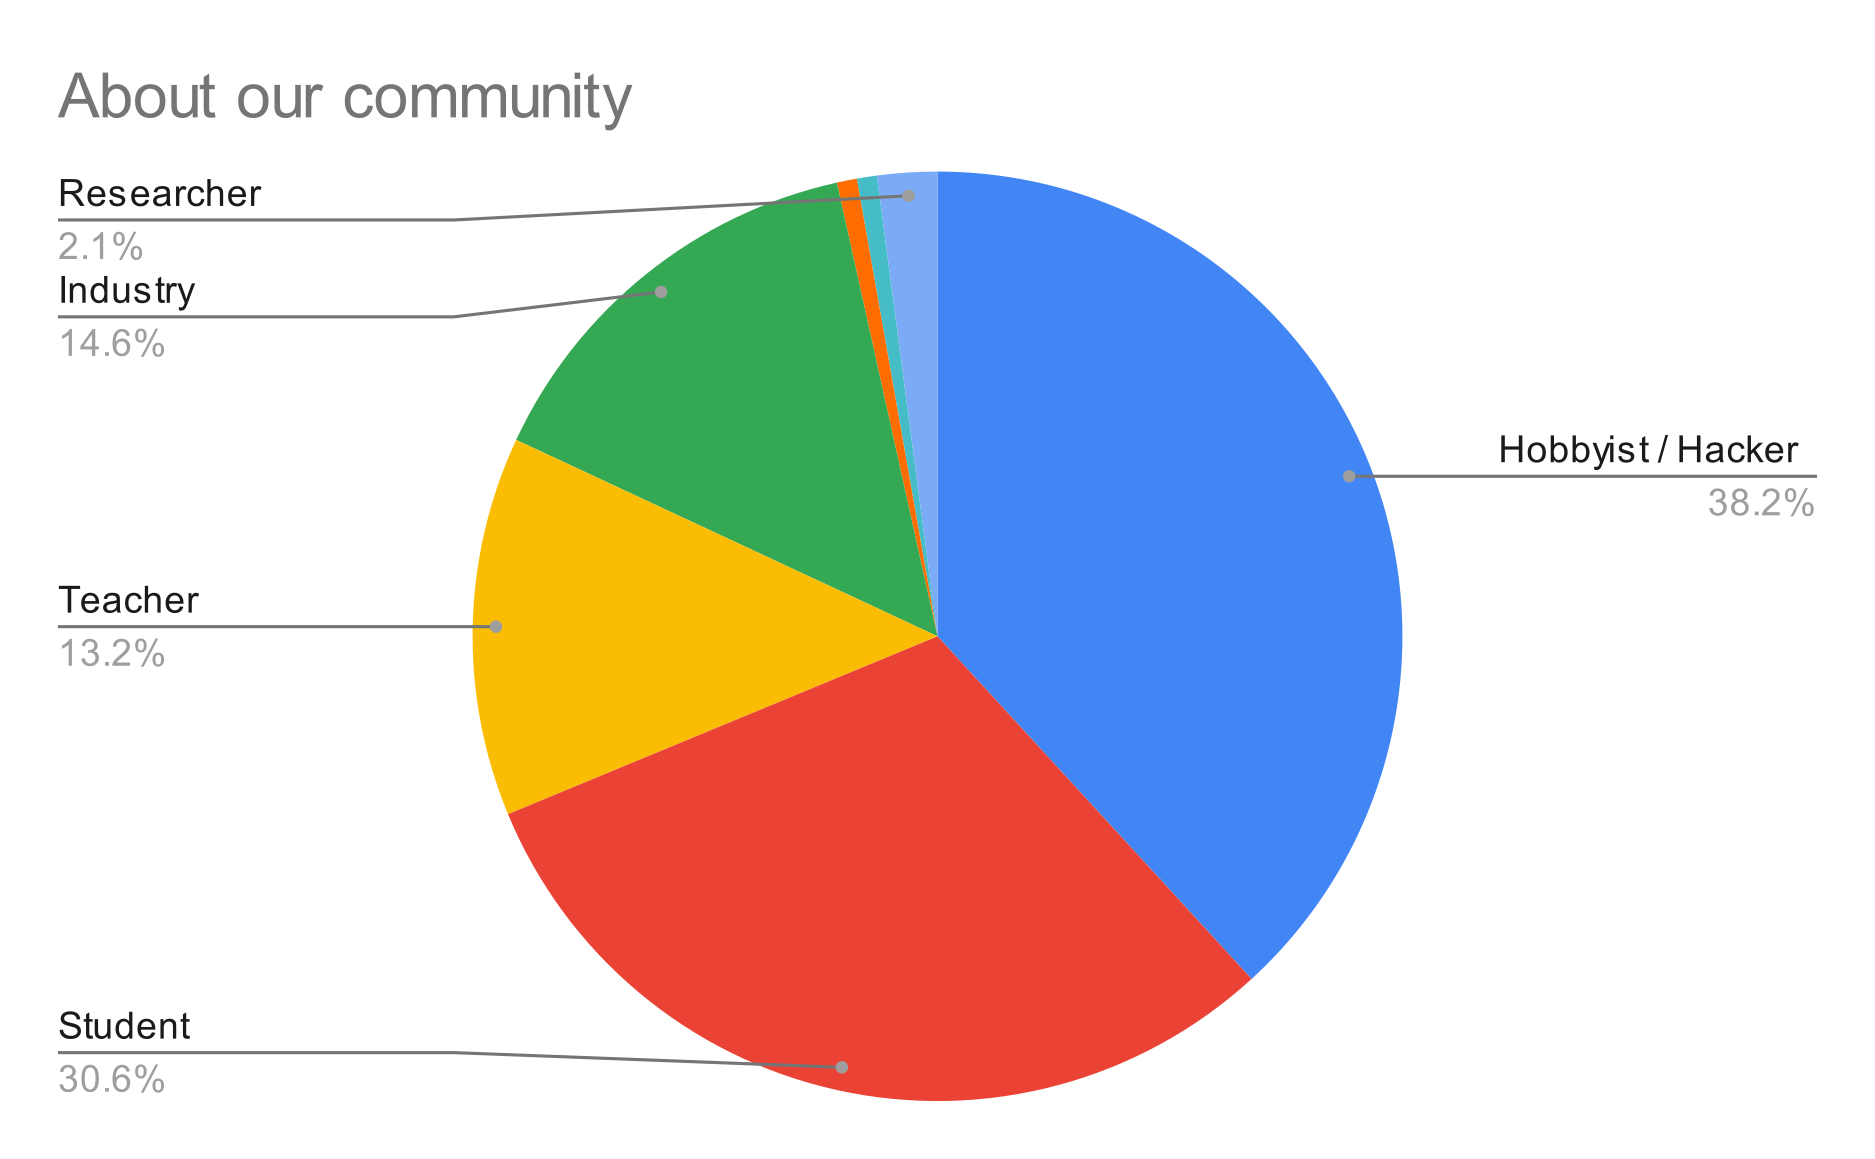
\includegraphics[width=\columnwidth]{./Figs/about our community pie chart.png}
\caption{How TT04 submitters identified themselves.}
\label{fig:TT02_submitters}
\end{figure}
